\subsection{LQGI zur Disturbance Rejection}
    Eine unbekannte Störung $w(t)$ wirkt additiv auf den Eingang $u(t)$ von $P(t)$ (kann auch an anderen Stellen angreifen. Ist für LQGI egal) aber nicht auf den Beobachter.
    
    Wir führen einen neuen Zustand für das System ein:
    \begin{align*}
        v(t) &= \int_0^t \big(0-y(\tau)\big)d\tau\\
        \Tilde{x}(t) &= \begin{bmatrix}x(t)\\\widehat{x}(t)\\v(t)\end{bmatrix},\quad \Tilde{x}(t)\in\mathbb{R}^{2n+m}
    \end{align*}
    Das Eingangssignal erweitert sich zu
    \begin{equation*}
        -K\cdot\widehat{x}(t) + K_I\cdot v(t),
    \end{equation*}
    wobei die Varibalen $K,\, K_I$ aus der LQRI-Formulierung stammen:
    \begin{gather*}
        \{\Tilde{A},\Tilde{B},\Tilde{Q},R\}\rightarrow \Tilde{K}= [K,-K_I]\\
        \Tilde{A}=\begin{bmatrix}A & 0\\ -C & 0\end{bmatrix},\quad \Tilde{B} = \begin{bmatrix}B\\0\end{bmatrix},\quad \Tilde{Q} = \begin{bmatrix} Q & 0\\ 0 & \gamma\cdot I\end{bmatrix}
    \end{gather*}
    Je Tiefer $\gamma$, desto langsamer das Integratorverhalten.
    
    \begin{figure}[H]
        \centering
        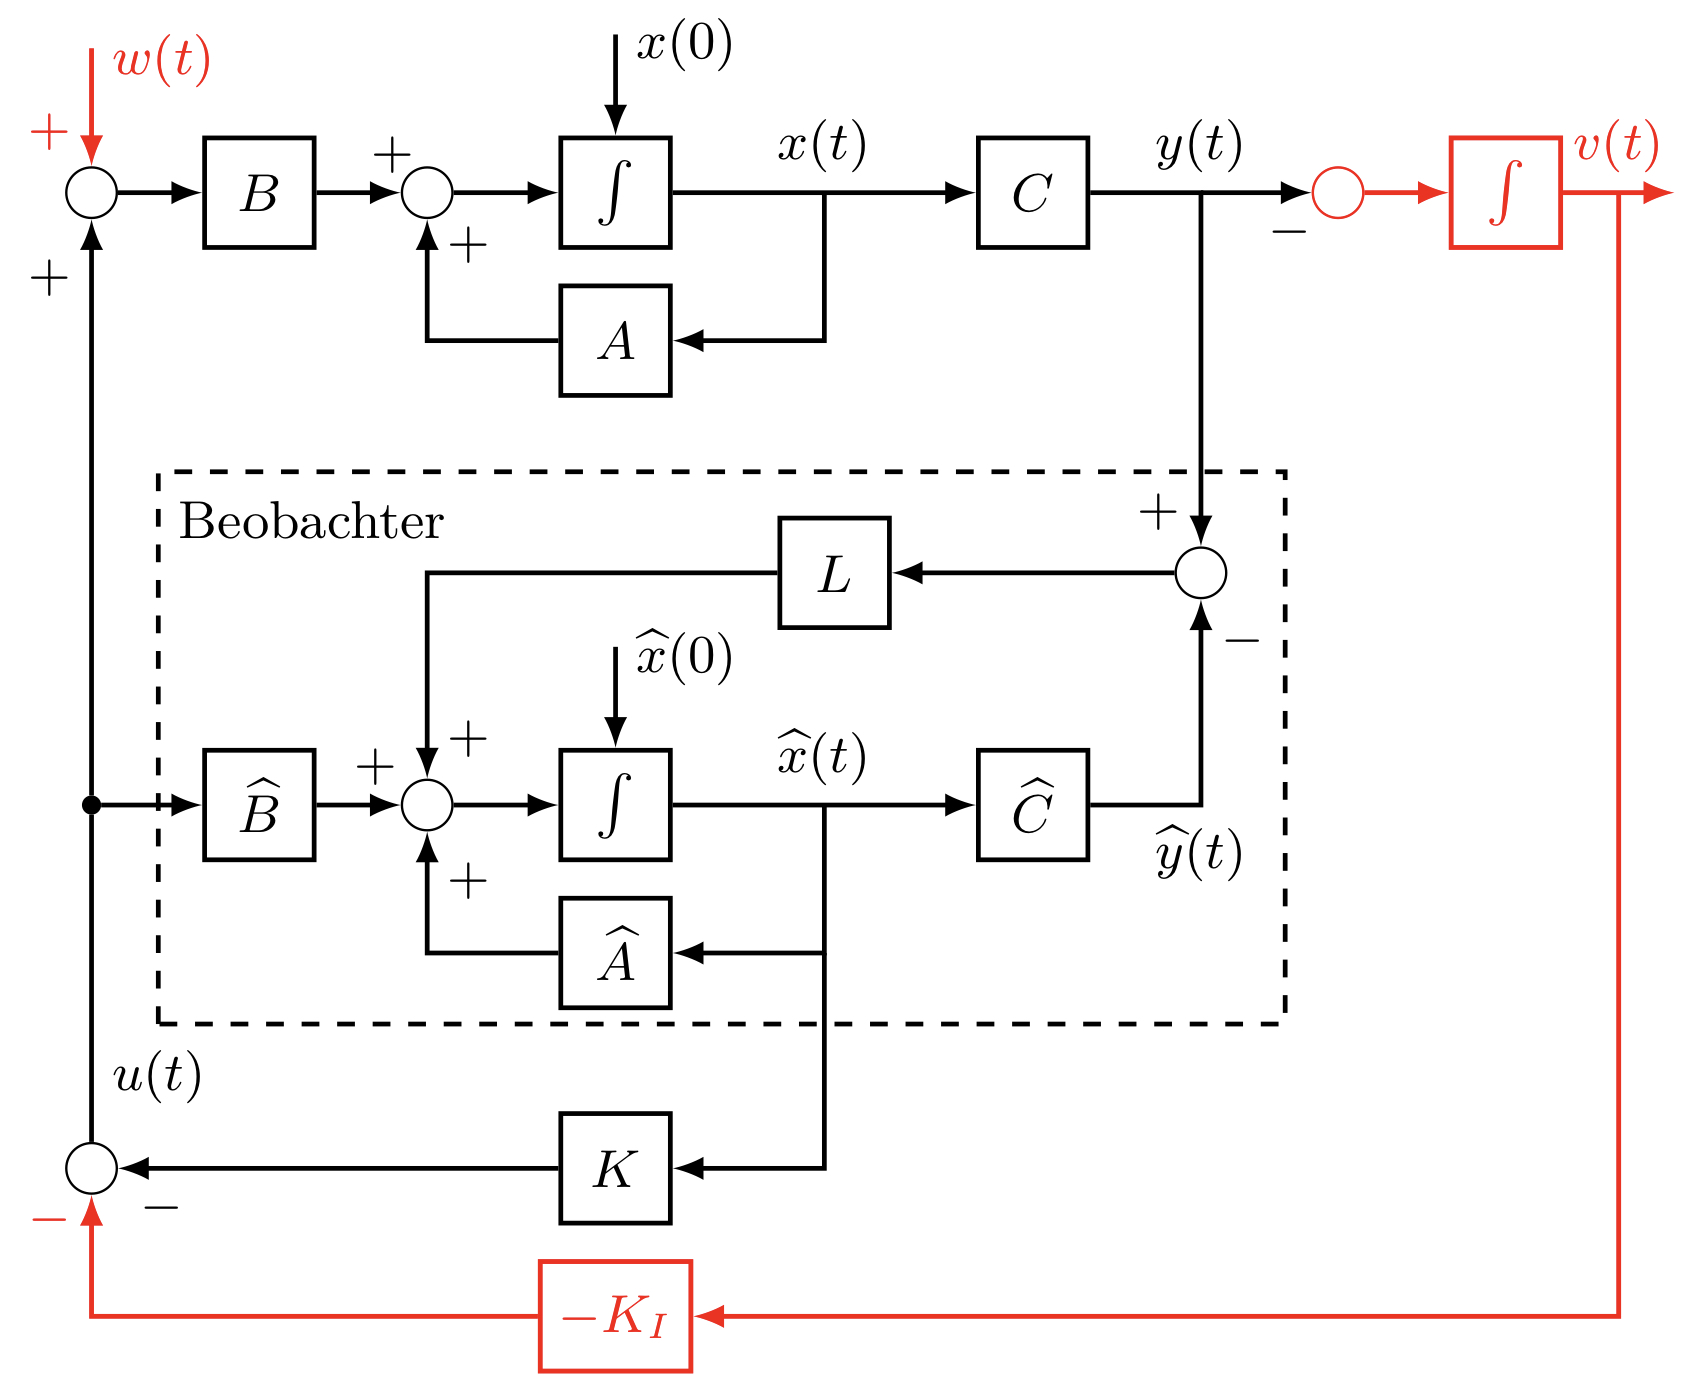
\includegraphics[width = 0.7\linewidth]{images/10/LQGI_distrejec.jpeg}
        \caption{Blockdiagramm für LQGI mit Störungsunterdrückung}
    \end{figure}
    
    \begin{figure}[H]
        \centering
        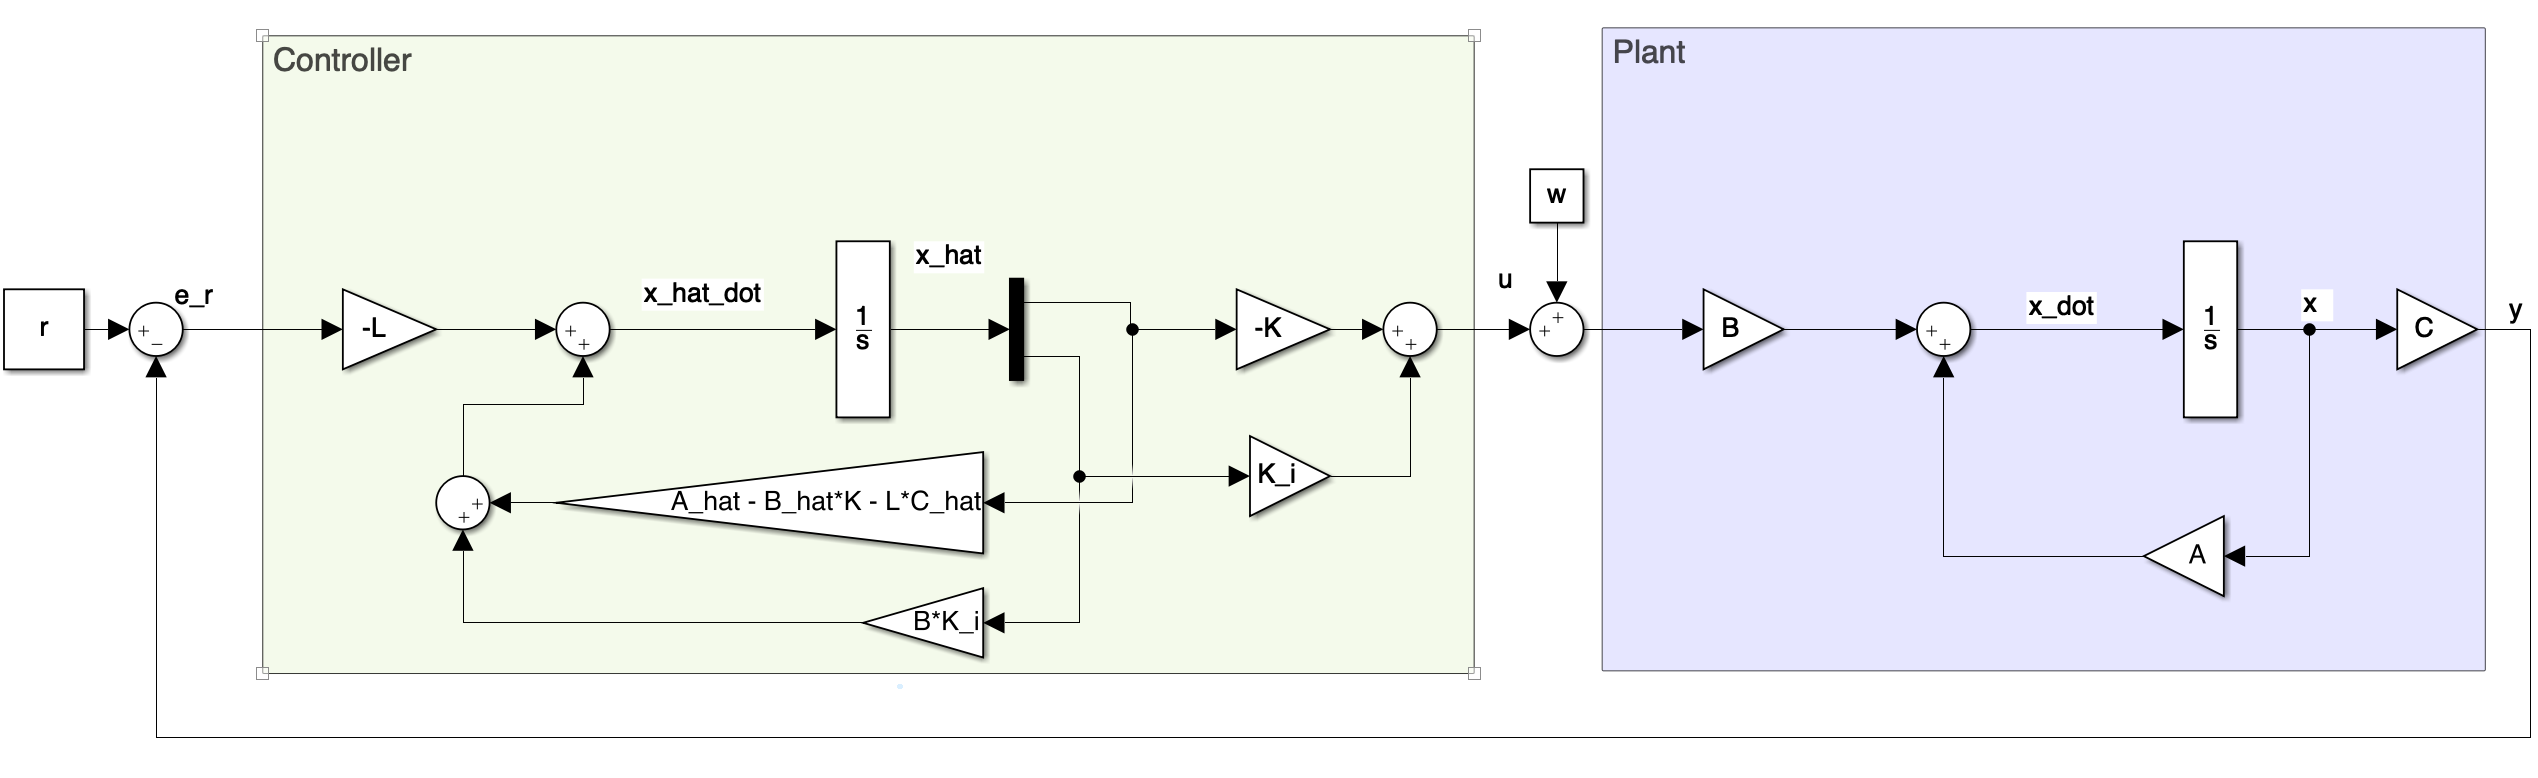
\includegraphics[width = \linewidth]{images/10/LQGI_alt.png}
        \caption{Alternative Dastellung des LQGI Reglers.}
        \label{fig:lqgialt}
    \end{figure}
    In dieser Darstellung von Abb. \ref{fig:lqgialt} enstpricht $\Tilde{x} = \begin{bmatrix}\widehat{x} \\ v\end{bmatrix}$ und $-L = \begin{bmatrix}-L\\ I \end{bmatrix}$. Die Dynamik des Observers ist dadurch gegeben als:
    \begin{align*}
        \Dot{\Tilde{x}}(t) &= \begin{bmatrix} \widehat{A}-\widehat{B}K - L\widehat{C} & BK_I\\
        0 & 0
        \end{bmatrix}\Tilde{x} + \begin{bmatrix} -L \\ I \end{bmatrix} e \quad (e = r-y = -y)\\
        u &= \begin{bmatrix} -K & K_I \end{bmatrix}\Tilde{x}
    \end{align*}
        
\subsection{LQGI mit Folgeregelung}
    LQGI mit Folgeregelung folgt aus der Kombination der beiden Ansätze. Dabei änder sich der Zustand $v(t)$ zu
    \begin{equation*}
        v(t) = \int_0^t \big(r(\tau)-y(\tau)\big)d\tau.
    \end{equation*}
    Das Eingangssignal resultiert als:
    \begin{equation*}
        u(t) = \mathit{\Gamma}\cdot r(t) - K \cdot\widehat{x}(t)+K_I\cdot v(t),
    \end{equation*}
    wobei $ \mathit{\Gamma}$ Gleich definiert ist wie in Abschnitt \ref{s:LQGIFolgeregelung}.
    
    \begin{figure}[H]
        \centering
        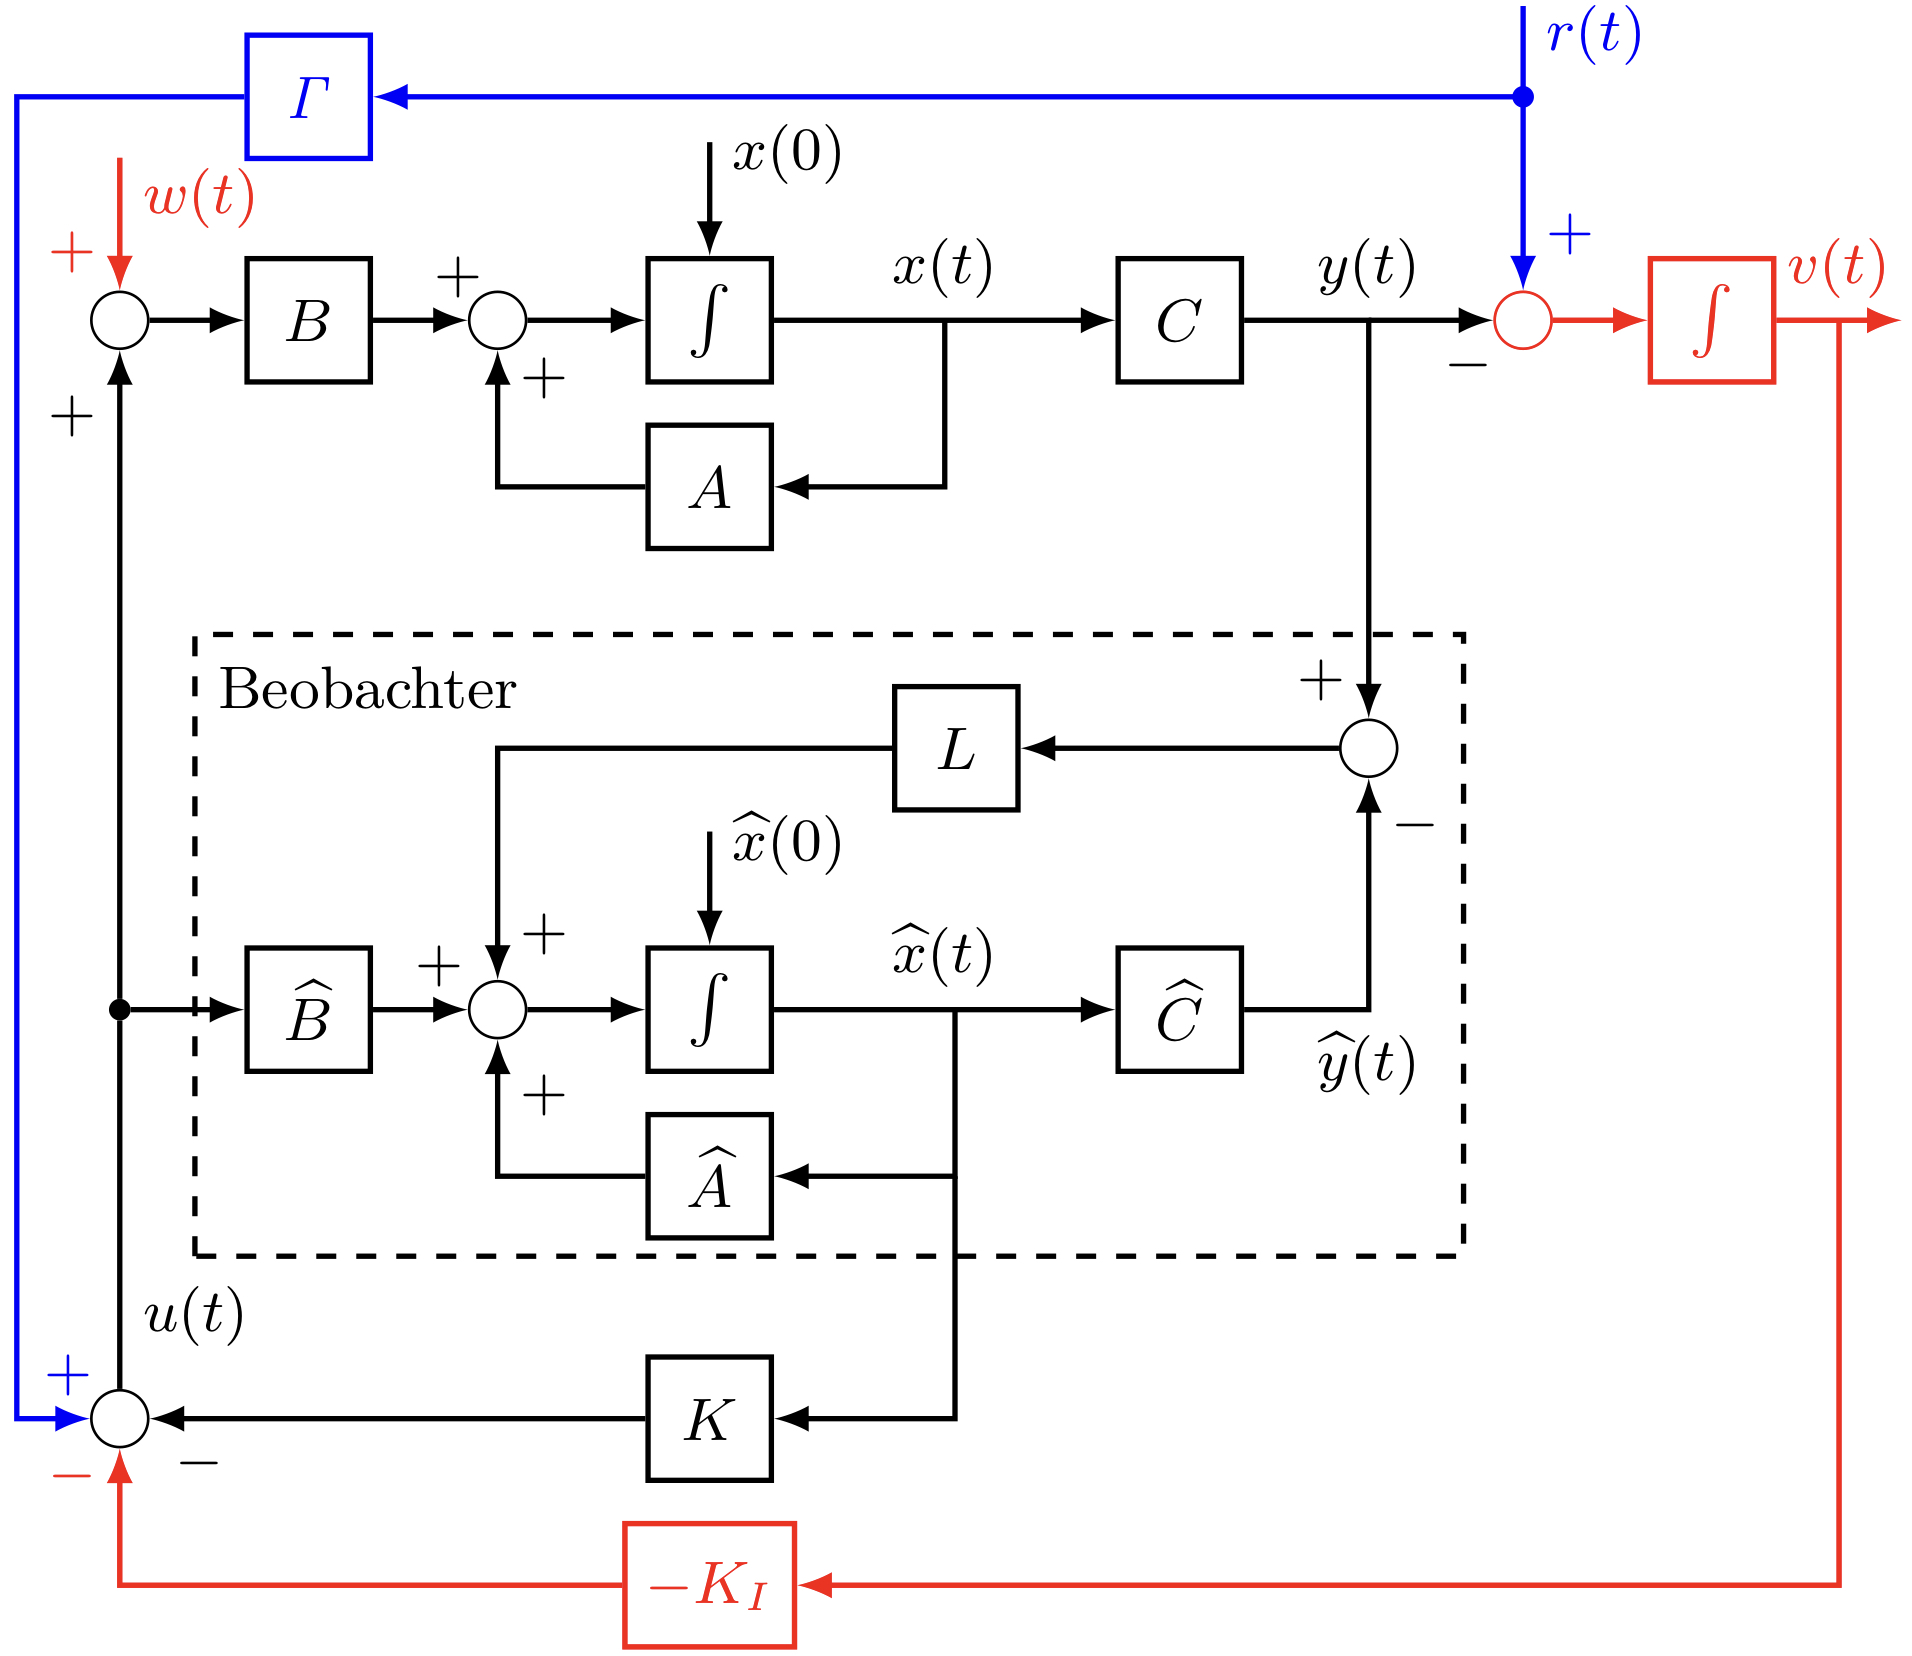
\includegraphics[width = 0.7\linewidth]{images/10/LQGI_Vorstr.jpeg}
        \caption{LQGI mit Vorsteuerung}
    \end{figure}
    
    \subsubsection{Auslegungsvorgehen}
        Die Auslegung eines LQGI-Reglers mit Folgeregelung verläuft nach diesem Rezept:
        
        \begin{enumerate}
            \item LQRI-Regler designen: $\{\Tilde{A},\Tilde{B},\Tilde{Q},\Tilde{R}\}\rightarrow \Tilde{K} = [K, -K_I]$, dabei werden $\Tilde{Q},\, R$ iterativ eingestellt
            
            \item Obersever designen: $\{A^\top, C^\top,\Bar{B}\cdot\Bar{B}^\top,q\cdot I\}\rightarrow L^\top$, dabei werden $\Bar{B},\, q$ iterativ eingestellt.
            
            \item Hinzufügen der Vorsteuerung für die Folgeregelung über die Matrix $\mathit{\Gamma}$.
        \end{enumerate}